\documentclass[spanish]{beamer}
\usepackage{lmodern}
\usepackage[T1]{fontenc}
\usepackage[utf8]{inputenc}
\usepackage{babel}

\usepackage{graphicx,hyperref,ru,url,bm}

\setbeamertemplate{caption}{\raggedright\insertcaption\par}

\def\realR{\mathbb{R}} % Defines the way to use real numbers symbol R.

% The title of the presentation:
%  - first a short version which is visible at the bottom of each slide;
%  - second the full title shown on the title slide;
\title[Espacios Tangentes]{
    Espacios Tangentes}

% Optional: a subtitle to be dispalyed on the title slide
\subtitle{El concepto abstracto de curva en $\realR^{2}$ y variedad en $\realR^{n}$}

% The author(s) of the presentation:
%  - again first a short version to be displayed at the bottom;
%  - next the full list of authors, which may include contact information;
\author[Joaquín González Cervantes]{
  Joaquín González Cervantes \\\medskip
  {\small \url{joaquin@yandex.com}}}

% The institute:
%  - to start the name of the university as displayed on the top of each slide
%    this can be adjusted such that you can also create a Dutch version
%  - next the institute information as displayed on the title slide
\institute[Universidad de Guadalajara]{}

% Add a date and possibly the name of the event to the slides
%  - again first a short version to be shown at the bottom of each slide
%  - second the full date and event name for the title slide
\date[\today]{
   \today}

\begin{document}

\begin{frame}
  \titlepage
\end{frame}

% Section titles are shown in at the top of the slides with the current section 
% highlighted. Note that the number of sections determines the size of the top 
% bar, and hence the university name and logo. If you do not add any sections 
% they will not be visible.
\section{Introducción}

\begin{frame}
\frametitle{¿De qué trata?}

  \begin{block}{}
    \begin{itemize}
        \item Definir el concepto de variedad $k$-dimensional en $\realR^{n}$ y su espacio tangente asociado a un punto.
        \item Determinar la dimensi\'on de $T_{p}N$.
        \item Interpretar una curva en el plano como un caso especial de variedad utilizando el Teorema de la Funci\'on Impl\'icita.
        \item Analizar el espacio tangente de una curva como un caso particular del espacio tangente asociado a una variedad.
    \end{itemize}
  \end{block}
\end{frame}

\begin{frame}
    \frametitle{Surge el vector}
    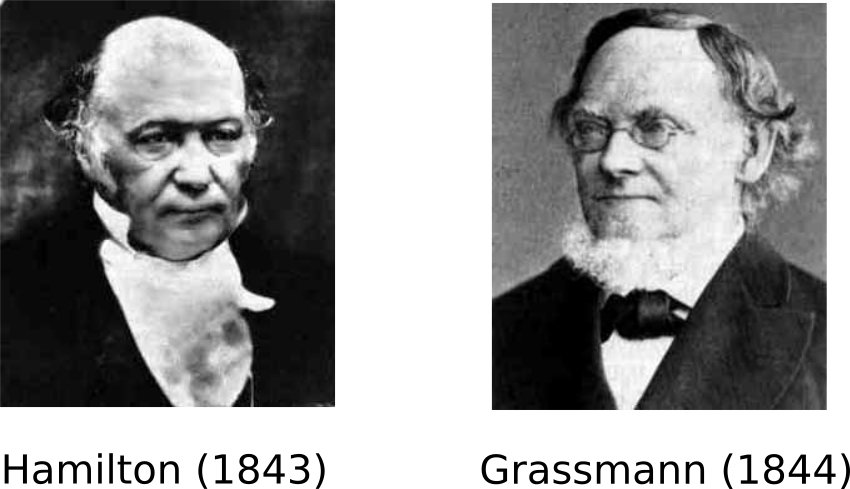
\includegraphics[width=\textwidth]{../gfx/hamilton-grassmann}
\end{frame}

\section{Curvas}

\begin{frame}
    \begin{definition}
        Una curva parametrizada en $\realR^{3}$ es una mapeo 
        $$c:I \rightarrow \realR^{3}$$
        para alg\'un intervalo abierto $I$.
    \end{definition}
\end{frame}

\begin{frame}
    \frametitle{Caracol de Pascal}
    El caracol de Pascal es la curva parametrizada
    $$ c(t)=((1+2\cos{t})\cos{t},(1+2\cos{t})\sin{t})\text{,} \quad t \in \realR$$
    El vector tangente es
    $$ c'(t)=(-\sin{t}-4\cos{t}\sin{t},\cos{t}+4\cos^{2}{t}-2)$$
    En particular,
    $$ c'(\pi/4) = (-\frac{\sqrt{2}}{2}-2,\frac{\sqrt{2}}{2})$$
\end{frame}

\begin{frame}
    \frametitle{Caracol de Pascal}
    \begin{columns}
    \column{0.5\textwidth}
        \begin{center}
            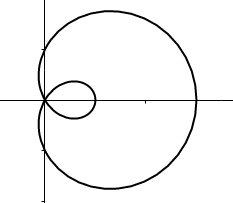
\includegraphics[scale=0.5]{../gfx/limacon2}
        \end{center}
    \column{0.5\textwidth}
        \begin{center}
            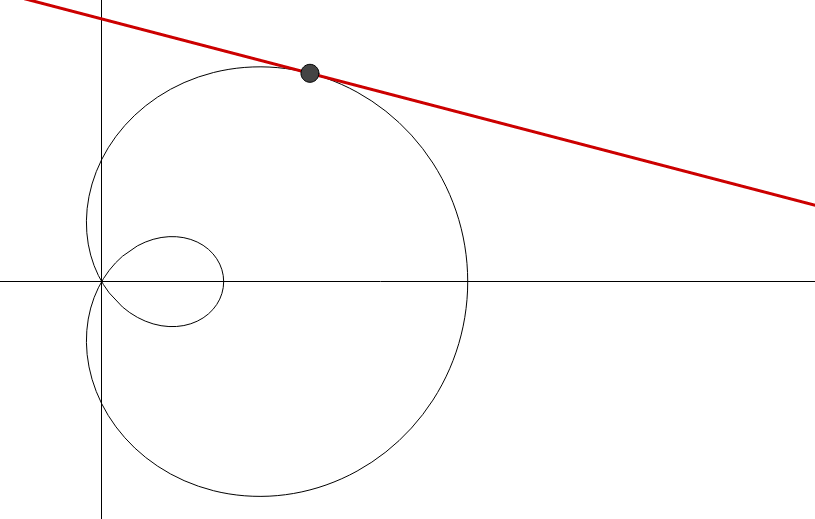
\includegraphics[scale=0.5]{../gfx/limacon}
        \end{center}
    \end{columns}
\end{frame}


\section{Subvariedad}
\begin{frame}
    \frametitle{Teorema de la funci\'on impl\'icita}
    \begin{columns}
    \column{0.5\textwidth}
        \begin{center}
            \includegraphics[scale=0.3]{../gfx/unit-circle1}
        \end{center}
    \column{0.5\textwidth}
        \begin{center}
            \includegraphics[scale=0.3]{../gfx/unit-circle2}
        \end{center}
    \end{columns}
\end{frame}

\begin{frame}
    \begin{figure}[ht]
      \begin{center}
      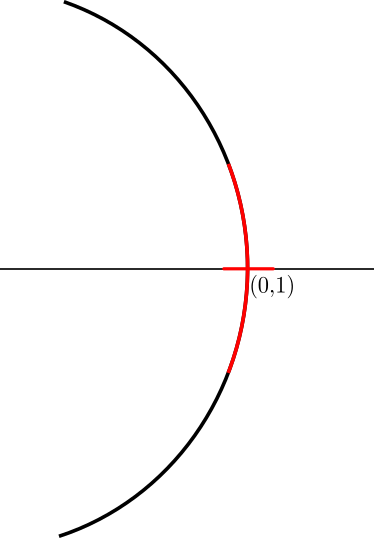
\includegraphics[width=0.5\linewidth]{../gfx/unit-circle3}
      \end{center}
    \end{figure}
\end{frame}

\begin{frame}
    \begin{theorem}[Teorema de la funci\'on impl\'icita]
        Sea $\bm{x} = (x_{1},x_{2},\ldots,x_{n})$ y sea $F(\bm{x},y) \in C^{1}$ 
        en una vecindad de $(\bm{x_{0}},y_{0})$ tal que
        \begin{enumerate}
            \item $F((\bm{x_{0}},y_{0})) = 0$
            \item $\frac{\partial F}{\partial y}((\bm{x_{0}},y_{0})) \ne 0$
        \end{enumerate}
        entonces existe una vecindad de $(\bm{x_{0}},y_{0})$ en donde existe una
        funci\'on \'implicita $y=f(\bm{x})$ tal que
        \begin{enumerate}[i.]
            \item $f(\bm{x_{0}}) = y_{0}$
            \item $F(\bm{x}, f(\bm{x})) = 0$
            \item $\frac{\partial f}{\partial x_{i}} = -\cfrac{\cfrac{\partial F}{\partial x_{i}}(\bm{x},f(\bm{x}))}{\cfrac{\partial F}{\partial y}(\bm{x},f(\bm{x}))}$
        \end{enumerate}
    \end{theorem}
\end{frame}

\begin{frame}
    \begin{definition}[Espacio tangente a $\realR^{n}$]
        Para cada punto $x \in \realR^{n}$ el espacio
        $$ T_{x}\realR^{n} := \{x\} \times \realR^{n} $$
        es llamado el espacio tangente en el punto $x$ (el espacio de todos los vectores
        tangentes en el punto $x$). La derivada (o diferencial) $Df$ de un mapeo diferenciable
        $f$ est\'a definido como
        $$ Df|_{x}: T_{x}\realR^{k} \rightarrow T_{f(x)}\realR^{n} \quad \text{con} \quad
        (x,v) \mapsto (f(x),J_{x}f(v)) \text{.} $$
    \end{definition}
\end{frame}

\begin{frame}
    \begin{definition}\label{def:immersion}
        Una inmersi\'on es un mapeo diferenciable entre variedades donde su
        derivada es inyectiva. Expl\'icitamente, $f:M \rightarrow N$ es una inmersi\'on si
        $$ D_{p}f: T_{p}M \rightarrow T_{f(p)}N $$
        es un mapeo inyectivo para toda $p \in M$. De forma equivalente, $f$ es una inmersi\'on
        si su derivada tiene rango igual a dim $M$:
        $$ rank D_{p}f = \text{dim }M \text{.} $$
    \end{definition}
\end{frame}

\begin{frame}
    \begin{definition}[Espacio tangente a una variedad]
        Sea $M \subset \realR^{n}$ una variedad k-dimensional, y sea $p \in M$. El
        espacio tangente a $M$ en el punto $p$ es el subespacio vectorial $T_{p}M \subset T_{p}\realR^{n}$,
        el cual se define como
        $$ T_{p}M := Df_{u}(\{u\} \times \realR^{k})=Df_{u}(T_{u}\realR^{k}) $$
        para una parametrizaci\'on $f:U \rightarrow M$ con $f(u) = p$, donde $U \subset \realR^{k}$ es
        un conjunto abierto.
    \end{definition}
\end{frame}
\end{document}
